\documentclass[12pt,a4paper,titlepage]{article}
\usepackage[utf8]{inputenc}
\usepackage[english]{babel}
\usepackage{amsmath}
\usepackage{amsfonts}
\usepackage{amssymb}
\usepackage{graphicx}
\usepackage[left=2.50cm, right=2.50cm, top=2.50cm, bottom=2.50cm]{geometry} 
\newtheorem{definition}{Definition}
\newtheorem{example}{Example}[section]
\newtheorem{theorem}{Theorem}[section]
\usepackage{enumerate}
\usepackage{tabularx, booktabs, colortbl, csquotes, hyperref, listings, pdfpages, paralist, xcolor}
\usepackage{placeins}
\setlength{\parindent}{1.5cm}
\pagestyle{plain}
\usepackage{tocloft}
\usepackage{apacite}
%hpenation stop
\tolerance=1
\emergencystretch=\maxdimen
\hyphenpenalty=10000
\hbadness=10000
\sloppy
\usepackage[nohyperlinks]{acronym}
\usepackage{setspace, latexsym}
\doublespacing
\author{Joseph Baafi}
\title{Modelling the Effect of Climate on Mosquito Population Dynamics and Malaria Spread with Controls.}
\begin{document}
\maketitle
\tableofcontents
%\date{}
\newpage
\section{Statement of Purpose} 

Mosquitoes remain one of the most efficient vectors of human and animal diseases and are responsible for transmitting some of the deadly diseases such as malaria and Dengue \cite{beck2013effect, abdelrazec2017mathematical, hamdan2020effect, abiodun2016modelling}. Transmission of these diseases depend on the age-structure and population abundance of female adult mosquitoes.  Malaria is the most prevalent human vector borne disease, with one half of the world population living in areas where malaria is endemic \cite{WikBlack5}.

 Mosquito’s developmental stages are known to depend on climatic conditions such as temperature, rainfall, wind and humidity \cite{agusto2015qualitative, mordecai2013optimal, abdelrazec2017mathematical}. Several models have been used to predict mosquito population dynamics in the presence of climate change \cite{beck2013effect, abdelrazec2017mathematical, hamdan2020effect}. However, a higher percentage of the existing models were formulated to study the population dynamics of a specific mosquito species within a specific geographical area \cite{agusto2015qualitative, mordecai2013optimal, abiodun2016modelling, abdelrazec2017mathematical} and so may not be applicable to other species or geographical areas. A few models have been developed to study general mosquito species. Controlling mosquito population has been an important issue for governments, since they cause diseases to humans and other organisms. Improved understanding of population dynamics and better management strategies would reduce the cost of treatment of diseases caused by mosquitoes ie. Malaria, Dengue and so on and  the reduce overwhelming in the hospitals in some temperate regions in Africa.  

Much work have not been done to compare how regional climate affects mosquito population dynamics, stage structure and control or management \cite{hurford2019regional}.
This project will develop a stage-structured non-autonomous ordinary differential equation model to study mosquito population dynamics in different regions with strong temperature and rainfall fluctuations.
Thus, this project seeks to modify and improve current models’ ability to model the population dynamics of mosquitoes. It also seeks to analyse the effects of regional variation in climate on population dynamics and stage structure of mosquitoes. The model will also seek to analyse some region-specific management strategies such as application of larvicides and adulticides. This work also seeks to address questions as, what time of the year should controls be implemented to control or eradicate the mosquitoes?. We also analyse the effectiveness of proper drainage systems, use of treated bed nets in controlling mosquito population.

\section{Background and Justification}
Malaria is a life-threatening disease caused by parasites that are transmitted to people through the bites of infectious female Anopheles mosquitoes \cite{WikBlack5, beck2013temperature}. It is estimated that there were 228 million cases of malaria worldwide with 405 000 deaths in 2018 \cite{WikBlack5}. In 2018, nearly half of the world's population was at risk of malaria with most cases and deaths occurring in sub-Saharan Africa \cite{WikBlack5}.
 
Vector control is the main way to prevent and reduce malaria transmission \cite{WikBlack5}. The reduction of human-vector contacts reduces the population density of vectors and hence, malaria transmission. Several vector management strategies have been implemented over the years and have proved to be effective in providing protection against infection \cite{Ocspp2016SuccessIM}. Mosquito breeding source reduction and management remain effective strategies for malaria vector control \cite{Ocspp2016SuccessIM}.

The mosquito model establishes the population abundance of both the juvinile and adult mosquitoes and deepen our understanding on the impact of climate on mosquito population dynamics. This also highlight the importance of incorporating detail vector biology into models for predicting mosquito population abundance and the risk of malaria incidence \cite{beck2013effect, beck2017importance}. Also the mosquito-human malaria model provides the framework for analysis of controls. 

\section{Goals and Objectives}
%The  main goals  of  this  project  is to  shapen  our  understanding  of the  effect  of temperature and rainfall on mosquito population and  to  analyze  the effectiveness of control strategies such as lavicides and adulticides through the development of ordinary differential equation models.

The goal of this project is to build a temperature and rainfall dependent, stage-structured ordinary differential equation model based on \cite{abdelrazec2017mathematical, hamdan2020effect, ewing2016modelling} to better understand how climate affects mosquito abundance and determines risk of malaria incidence. 

Mosquito life stages are strongly dependent on temperature and rainfall and several studies have been able to predict mosquito population abundance. Most of these studies are done on special mosquito species and a given geographical areas. Hence, general mosquito models can be improved. 

Thus, this project has for it objectives;

\begin{itemize}
\item To develop a stage-structured population model that incorporate temperature and rainfall.
\item To predict mosquito abundances and malaria risk according to regional climate patterns.
\item To analyze the effect of control measures at the various life stages of mosquito.
\item To compare the effectiveness of controls and to estimate the best periods where controls will be effective. 
\item To build a combined mosquito-human malaria transmisson model to analyze how climate determines risk.  
\end{itemize}


\section{Methods}
We develop a stage-structured ordinary differential equation model based on \cite{abdelrazec2017mathematical, hamdan2020effect, abiodun2016modelling, ewing2016modelling} to emphasize the impact of temperature and rainfall on mosquito population dynamics. The novelty in seen in the fact that natural mortality rate at the various life stages are introduced and different regions leading to different climate patterns will be studied. The basic reproduction number of both the autonomous and the non-autonomous models will be studied and used to analyze controls in the autonomous system. Sensitivity of the model to parameters will be analyzed through sensitivity analysis. 

Also, the mosquito population model is modified to incorporate control strategies. We will analyze the effectiveness of larvicides and adulticides and estimate the correct times where implementation of controls will be much effective \cite{Ocspp2016SuccessIM}.

Again, we extend the non-automous mosquito model to include human compartments to explore the impact of climate variability on the incidence of malaria in different regions. sensitivity of the model to climate-dependent parameters will be analyzed to establish how climate influences parameters to determine risk \cite{abiodun2016modelling}. 

Also, latency in malaria infections and it's impact on the disease dynamics will be analyzed using a delay differential equation version of the ordinary differential equation model.


\subsection{Model}
The framework of the stage-structured temperature and rainfall-dependent mosquito population model reflects details of the mosquito life-cycle \cite{abdelrazec2017mathematical, hamdan2020effect, beck2013effect, ewing2016modelling}. The model allows us to incorporate stage specific life history rate and process. The four main life stages that constitutes the stage structuring are eggs, larvae, pupae and adults. We assume that desity-dependence is only experienced in the larvae stage. Each life stage has a natural mortality as well as climate dependent mortality rate.  

The system of equations that describe the model are as follows:


\begin{subequations}
	\label{mosquito_model}
	\begin{align}
\dfrac{dE(t)}{dt} &= \phi (T, R)\left(1-\dfrac{A(t)}{K}\right)A(t) - \left( \delta_E(T, R)  + \pi_E(T, R)+ \mu_E\right)E(t)\\
\dfrac{dL(t)}{dt} &= \delta_E(T, R)E(t) - \left( \delta_L(T, R)  + \pi_L(T, R)+ \mu_L + \sigma_L L\right)L(t)\\
\dfrac{dP(t)}{dt} &= \delta_L(T, R)L(t) - \left( \delta_P(T, R)  + \pi_P(T, R)+ \mu_P \right)P(t)\\
\dfrac{dA(t)}{dt} &= \tau \delta_P(T, R)P(t) - \left( \pi_P(T, R)+ \mu_P \right)A(t)
	\end{align}
\end{subequations}

where $T = T(t)$ and $R=R(t)$ represent temperature and rainfall respectively. $T$ and $R$ are bounded periodic functions determined from climate data \cite{abdelrazec2017mathematical}.

A detailed description of all variables and parameters used in the model are given in Table \ref{tab:table1} and Table \ref{tab:table2} respectively. 

\begin{table}[h!]
	\begin{center}
		\caption{Description of variables used in the model \ref{mosquito_model}}
		\label{tab:table1}
		\begin{tabular}{l|l} % <-- Alignments: 1st column left, 2nd middle and 3rd right, with vertical lines in between
			\hline
			\textbf{Variables} & \textbf{Description} \\
			\hline
			$E(t)$ & Total number of eggs at  time t \\
			$L(t)$ & Total number of larvae at  time t \\
			$P(t)$ & Total number of pupae at  time t \\
			$A(t)$ & Total number of adults at  time t
			
		\end{tabular}
	\end{center}
\end{table}

\begin{table}[h!]
	\begin{center}
		\caption{Description of parameters used in the model \ref{mosquito_model}}
		\label{tab:table2}
		\begin{tabular}{l|l} % <-- Alignments: 1st column left, 2nd middle and 3rd right, with vertical lines in between
			\hline
			\textbf{Parameters} & \textbf{Description} \\
			\hline
			$\phi$ & Egg oviposition rate \\
			$\tau$ & Proportion of new adult female mosquitoes \\
			$K$ & Carrying capacity of the female adult mosquitoes \\
			$\delta_E(T, R)$ & Hatching rate of eggs \\
			$\delta_L(T, R)$ & Transition rate from larvae into pupae\\
			$\delta_P(T,R)$ & Transition rate from pupae into adult\\
			$\pi_E(T, R)$ & Climate-dependent mortality rate of eggs\\
			$\pi_L(T, R)$ & Climate-dependent mortality rate of larvae\\
			$\pi_P(T, R)$ & Climate-dependent mortality rate of pupae\\
			$\pi_A(T, R)$ & Climate-dependent mortality rate of adults\\
			$\mu_E$ & Natural mortality rate of eggs\\
			$\mu_L$ & Natural mortality rate of larvae\\
			$\mu_P$ & Natural mortality rate of pupae\\
			$\mu_A$ & Natural mortality rate of adults\\
			$\sigma_L$ & Density-dependent mortality rate of larvae\\
		\end{tabular}
	\end{center}
\end{table}

All parameter values used in the model will be based on data from lab studies and experimental results from \cite{bayoh2004temperature, bayoh2003effect, yang2011follow, esteva2015assessing}. 

%\tag{3.1}\label{eq:3.1}

\section{Potential Results}
\subsection{Analysis of the autonomous model}
The autonomous version of the model \ref{mosquito_model} is obtained by setting all the climate-dependent parameters to a constant and it is given by 

\begin{subequations}
	\label{autonomous_model}
	\begin{align}
		\dfrac{dE(t)}{dt} &= \phi\left(1-\dfrac{A(t)}{K}\right)A(t) - \left( \delta_E  + \pi_E+ \mu_E\right)E(t)\\
		\dfrac{dL(t)}{dt} &= \delta_EE(t) - \left( \delta_L  + \pi_L+ \mu_L + \sigma_L L\right)L(t)\\
		\dfrac{dP(t)}{dt} &= \delta_LL(t) - \left( \delta_P  + \pi_P+ \mu_P \right)P(t)\\
		\dfrac{dA(t)}{dt} &= \tau \delta_PP(t) - \left( \pi_P+ \mu_P \right)A(t)
	\end{align}
\end{subequations}

For this model \ref{autonomous_model} to make biological sense, the state variables as well as it's parameters must be non-negative for all time t. Thus, it can be studied in the invariant region: 
\begin{align}
D = \left\{ (E, L, P, A) \in R^4 : E, L, P, A \geq 0 \right\}.
\end{align}

Analysis of this model \ref{autonomous_model} indicates that the threshold quantity, $R_m$ given by 
\begin{equation}
	\label{R_m}
	R_m = \frac{\tau\phi\delta_E\delta_L\delta_P}{(\mu_A+\pi_A)(\delta_P+\mu_P+\pi_P)(\delta_L+\mu_L+\pi_L + \sigma_L)(\delta_E+\mu_E+\pi_E)}.
\end{equation}

$R_m$ is the vectorial reproduction number also known as basic offspring number. It measures the average expected number of female adult offsprings produced by a single female mosquito during it's life time \cite{abdelrazec2017mathematical, hamdan2020effect}. 

\begin{figure}[!h]
	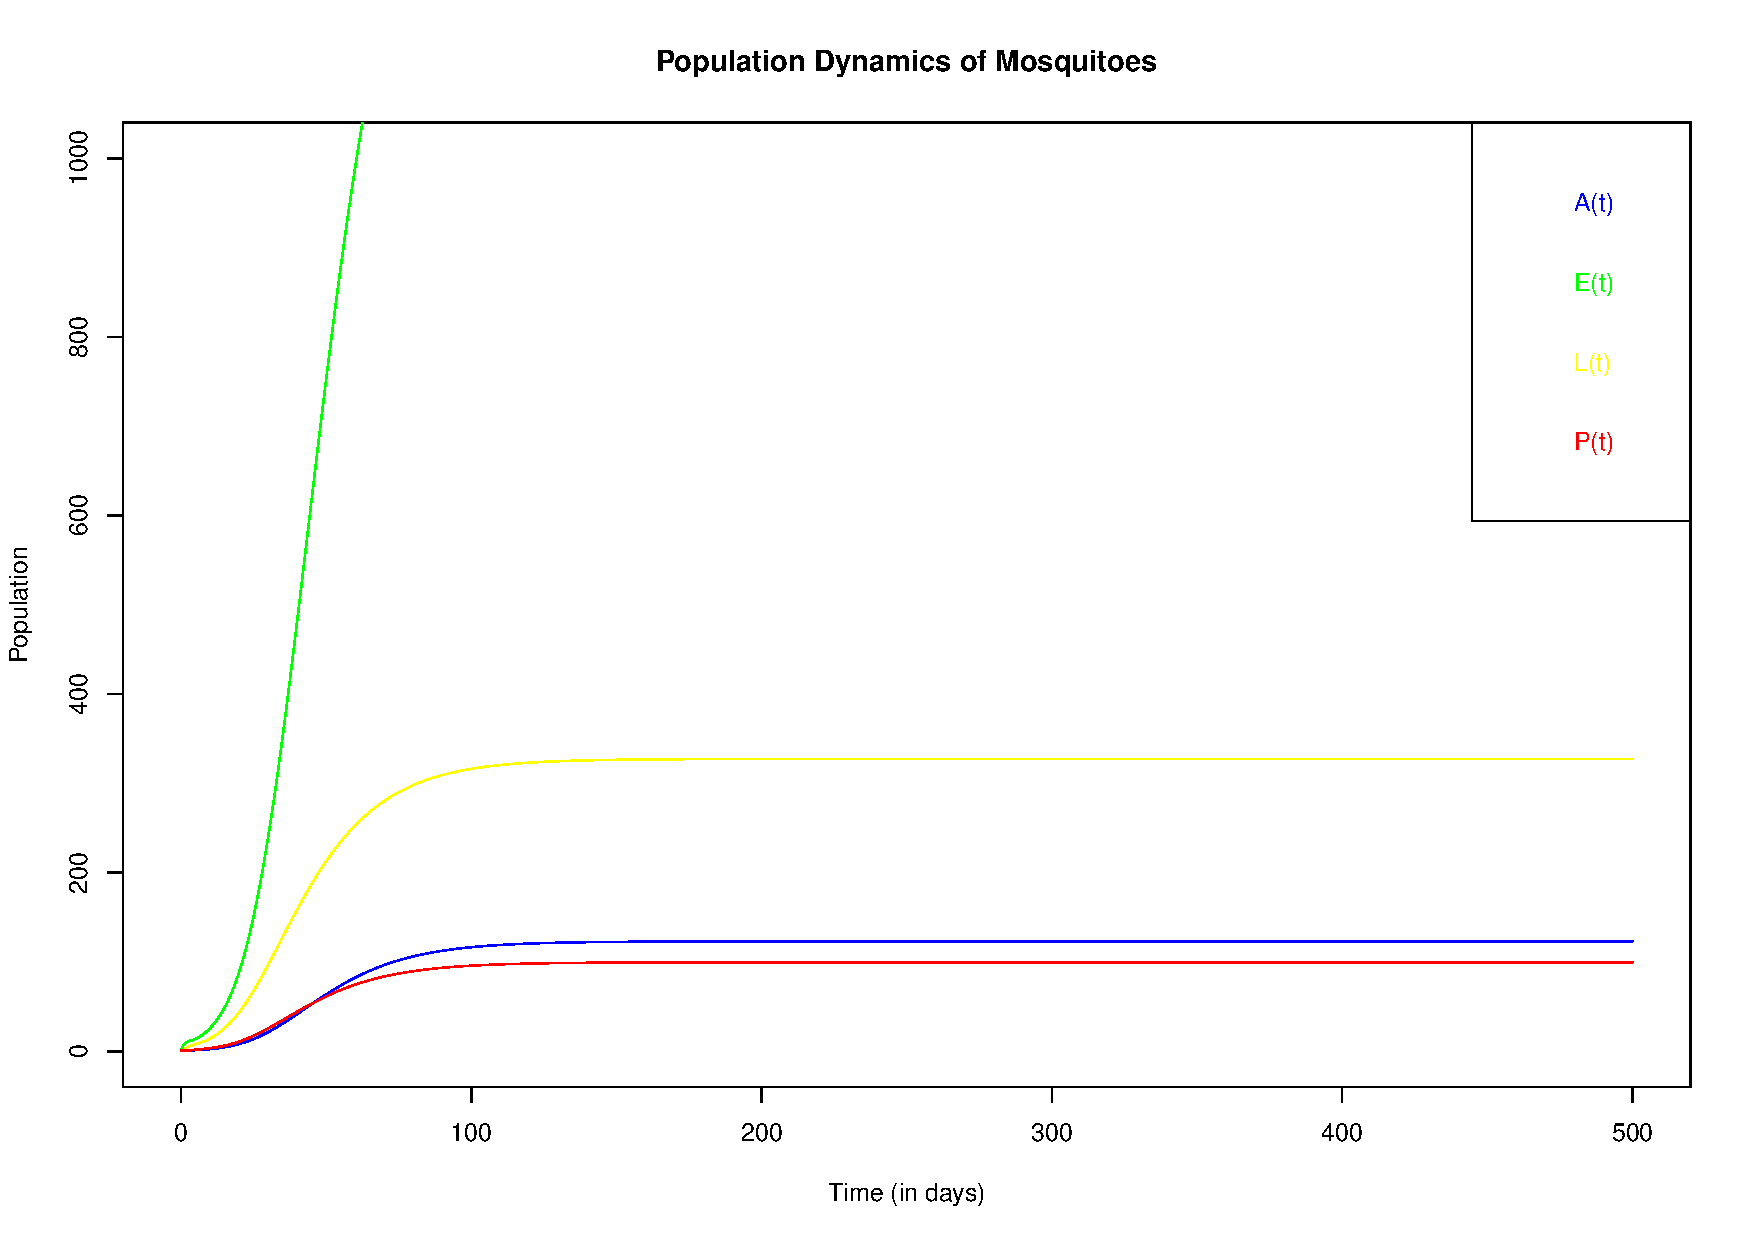
\includegraphics[width=0.8 \textwidth]{mosquito.pdf}
	\caption{Population Dynamics of mosquitoes obtained from \ref{autonomous_model} with $\phi = 10.7$, $K = 10^6$, $\delta_E = 0.4$, $\delta_L = 0.14$, $\delta_P = 0.3$, $\mu_E 0.36$, $\mu_L = 0.30$, $\mu_P = 0.15$, $\mu_A = 0.10$,   $\pi_E = 0.11$, $\pi_L = 0.10$, $\pi_P =  0.01$, $\pi_A = 0.07$, $\sigma_L = 0.004$, $\chi = 0.7$    
	\label{population_dynamics} 
\end{figure}

It is expected that the mosquito-malaria model will produce a reasonable fit with observe data. In particular, they will capture all the spikes in malaria prevalence. Our findings will further highlight the importance of climate on malaria transmission and show the seasonality of malaria epidemics. 



\section{Time table and Milestones}
This project begins with a literature review on mosquito life cycle and development, malaria transmission, climate effect on mosquito population, population models and control strategies in May 2020 and continues until October 2020. My research proposal writing begins in September 2020 and will be presented to the Memorial University Biology 7000 Graduate Core Seminar class. This proposal will be updated and presented to my thesis committee in  late January 2021. The baseline model for the first chapter of my thesis will be derived and analyzed in October and continues until April 2021. I expect to finish writing the first chapter of my thesis by May 2021. 




\bibliographystyle{apacite}
\bibliography{References}

\end{document}